\documentclass[fleqn]{jbook}
\usepackage{physpub}

\begin{document}

\begin{question}{専攻 問題2}{}

異なる媒質の境界面において、電磁波の満たす境界条件は一般に次のように与えられる。
\begin{equation}
E_t({\rm{I}})-E_t({\rm{II}})=0 \eqname{Q1}
\end{equation}
\begin{equation}
D_n({\rm{I}})-D_n({\rm{II}})=Q \eqname{Q2} 
\end{equation}
\begin{equation}
H_t({\rm{I}})-H_t({\rm{II}})=J \eqname{Q3}
\end{equation}
\begin{equation}
B_n({\rm{I}})-B_n({\rm{II}})=0 \eqname{Q4}
\end{equation}
ここに、$E$は電場、$D$は電束密度、$H$は磁場、$B$は磁束密度である。添字t、nは境界面に平行、垂直な成分をそれぞれ表わす。また、(I)、(II)は媒質を示し、$Q$は表面電荷密度、$J$は表面電流密度である。

\begin{subquestions}

\SubQuestion
マックスウェルの方程式とストークスの定理を用いて、式\eqhref{Q1}が成り立つことを示せ。

\SubQuestion
マックスウェルの方程式とガウスの定理を用いて、式\eqhref{Q2}が成り立つことを示せ。

\SubQuestion
媒質(II)が完全導体である場合、その表面において電磁波の満たすべき境界条件を求めよ。

\SubQuestion
媒質(I)が真空、媒質(II)が完全導体とする。真空側($x<0$)から導体面($yz$平面)に入射する平面波の電磁波を考える。この入射平面波は単色で$y$方向に偏光しており、
\begin{equation}
E_y=E_0\exp(-2\pi i\nu t+ikx) \eqname{Q5}
\end{equation}
で与えられるとする。ここに$\nu$は電磁波の振動数、$k$は波数である。これが金属表面($x=0$)で反射されるとき、導体面に流れる表面電流密度を求めよ。また、その方向を示せ。ただし、真空の誘電率と透磁率をそれぞれ$\varepsilon_0,\mu_0$とする。

\SubQuestion
次に、媒質(I)、(II)が異なる誘電体であるとする。これが、$yz$平面を境に互いに接している。ここに、$x<0$から\eqhref{Q5}式で与えられる平面波の電磁波が入射した。境界条件の式\eqhref{Q1}-\eqhref{Q4}を適用し、$x=0$の境界面における反射率(反射波と入射波の電場の比)、および、透過率(透過波と入射波の電場の比)をそれぞれ求めよ。ただし、媒質(I)の誘電率を$\varepsilon_1$、媒質(II)の誘電率を$\varepsilon_2$とし、透磁率はいずれも$\mu_0$とする。

\SubQuestion
平行な境界面をもつ誘電体の板が真空中に置かれている。その境界面に垂直な方向から電場の振幅が$E_0$である平面波の電磁波が入射する。平面波の振動数を$\nu$、板の厚さを$L$とするとき、この板を通過する電磁波の強度(ポインティングベクトルの大きさ)を求めよ。ただし、誘電体の誘電率を$\varepsilon_1$、真空の誘電率を$\varepsilon_0$とし、透磁率はいずれも$\mu_0$とする。

\SubQuestion
前問で、振動数$\nu$の電磁波に対して、透過する電磁波の強度が最大になるような$L$を求めよ。また、その時の透過強度の入射強度に対する比を求めよ。これらの結果についての物理的意味を考察し、簡潔に述べよ。以上の結果は、眼鏡の反射防止コーティングや干渉フィルターなどに広く応用されている。
\end{subquestions}
\end{question}
\begin{answer}{専攻 問題2}{}

\begin{subanswers}
\SubAnswer

\parbox[t]{100mm}{fig.1の微小長方形$ABCD$は、$AD,BC \ll AB,DC \ll 1 $を満た
すとする。マクスウェル方程式の一つ$\nabla\times \vec{E}=-\frac{\partial {\vec{B}}}{\partial t}$の両辺を図の長方形で積分し、左辺にStokesの公式を使うと、
\[\oint \vec{E} \cdot {\rm{d}}  {\vec{l}} = \int\nabla\times \vec{E}\cdot {\rm{d}} {\vec{S}} = -\frac{\partial}{\partial t}\int B\cdot {\rm{d}} S \]
となる。$AD \rightarrow 0, BC \rightarrow 0 $とすれば、
\[ \int_{AB} \vec{E}\cdot {\rm{d}}\vec{l} + \int_{CD} \vec{E}\cdot {\rm{d}}\vec{l} = 0 \]
を得る。$AB$も$CD$も$ \vec{E}$,境界面の変化に比べて短いので、
\[ E_t({\rm{I}})- E_t({\rm{II}})=0 \]
であることが分かる。}\parbox[t]{60mm}{\vspace*{-10mm}
\begin{center}
\includegraphics[clip,height=60mm,width=55mm]{1997phy2-1.eps}
\end{center}
}

\SubAnswer
\parbox[t]{100mm}{
fig.2の微小円柱(高さ $h$、底面積 $S$)において、$h \ll S \ll 1 $
である。$ D$ を円柱の表面で面積積分し、Gaussの公式と
マクスウェル方程式の一つ、$\Div D=\rho$を用いて変形すると下の式を得る。
\[\int {\vec{D}}\cdot {\rm{d}} {\vec{S}} = \int\nabla\cdot {\vec{D}} {\rm{d}}V
                         = \int\rho {\rm{d}}V                 \]
ここで、$h\rightarrow 0$とすると、
\[ ( {\vec{D}}({\rm{I}})- {\vec{D}}({\rm{II}}))\cdot \vec{S} = QS  \]
となる。$ {\vec{S}}$は、大きさ$S$で、円柱の底面の法線方向を向いたベクトル
である。$S$は $ {\vec{D}}$、境界面の変化に比べて小さい。従って、
\[  D_n({\rm{I}})-D_n({\rm{II}})=Q   \]
と結論できる。}\parbox[t]{60mm}{\vspace*{-10mm}
\begin{center}
\includegraphics[clip,height=60mm,width=55mm]{1997phy2-2.eps}
\end{center}
}

\SubAnswer
誘電率$\varepsilon$、透磁率$\mu$、電気伝導度$\kappa$の物質中での
マクスウェル方程式は、
\begin{equation}
\Rot \vec{E} = -\mu\frac{\partial {\vec{H}}}{\partial t} \eqname{Q6}
\end{equation}
\begin{equation}
\Rot \vec{H} = \varepsilon\frac{\partial \vec{E}}{\partial t}+\kappa \vec{E} \eqname{Q7}
\end{equation}
となる。完全導体中では、$\kappa\rightarrow\infty$である。このため
\eqhref{Q7}式の右辺第2項を見て、
\begin{equation}
 \vec{E} = 0  \eqname{Q8}
\end{equation}
\eqhref{Q6},\eqhref{Q8}より、
\[ \vec{H} = const. \eqname{Q9} \]
が分かる。$ H$が特になにかある値をとらなければならない理由は
ないので、const.=0 とする。
結局導体の内部では、
\[   \vec{E} = 0 \quad ,\quad    \vec{H} = 0  \]
となっている。問題に与えられた境界条件\eqhref{Q1}〜\eqhref{Q4}にこれらを代入すると、
\[ E_t({\rm{I}})=0 \quad ,\quad  D_n({\rm{I}})=Q \quad, \quad  H_t({\rm{I}})=J \quad,\quad B_n({\rm{I}})=0 \]
が得られる。

\SubAnswer

媒質(II)は完全導体で、表面電流密度、$ J = H_t({\rm{I}}) $
となる。マクスウェル方程式$\Rot E=-\mu_0\frac{\partial H}{\partial t}$に\eqhref{Q5}を代入すると、
\[ \Rot \vec{E} = \left(\begin{array}{c}
                   \partial_x \\
                   \partial_y \\
                   \partial_z
              \end{array}\right)\times
              \left(\begin{array}{c}
                     0   \\
                     E_y \\
                     0   
               \end{array}\right)=
               \left(\begin{array}{c}
                     0     \\
                     0     \\
                    i k E_0\exp(-2\pi i\nu t +  i kx)
               \end{array}\right)                 \]
であるから、これより
\[   \vec{H} = \left(\begin{array}{c}
                   0    \\
                   0    \\
          \frac{kE_0}{2\pi\nu\mu_0}\exp(-2\pi i\nu t+ i kx)
            \end{array}\right)    \]
となる。$H_x$、$H_y$が特別の値をとらなければならない理由はないので
これらの値は$0$とした。従って、
\begin{equation}
     H_z=\frac{kE_0}{2\pi\nu\mu_0}\exp(-2\pi i\nu t+ i kx)
  =\sqrt{\frac{\varepsilon_0}{\mu_0}}E_0\exp(-2\pi i\nu t+ i kx) \nonumber
\end{equation}
ただし、$k=2\pi\nu\sqrt{\varepsilon_0 \mu_0}$である。反射波$E_y',H_z'$については境界条件\eqhref{Q1},
$E_t({\rm{I}})=0$とマクスウェル方程式より、
\begin{equation}
  E_y'=-E_0\exp(-2\pi i\nu t- i kx) \quad , \quad H_z'=\sqrt{\frac{\varepsilon_0}{\mu_0}}E_0\exp(-2\pi i\nu t- i kx) \nonumber
\end{equation}
$x=0$として$H_z$と$H_z'$の和をとると、表面電流密度として、
\[  J=H_t(I)=H_z'+H_z=2\sqrt{\frac{\varepsilon_0}{\mu_0}}E_0\exp(-2\pi i\nu t)\]
が得られる。

\SubAnswer
入射波、反射波、透過波は
以下のように書ける。
\begin{eqnarray*}
入射波 : \quad E_y&=&E_0\exp(-2\pi i\nu t+ i kx)\quad ,\quad H_z=\sqrt{\frac{\varepsilon_1}{\mu_0}}E_y  \\
反射波 : \quad  E_y'&=&\mp E_0'\exp(-2\pi i\nu t- i k'x)\quad ,\quad H_z'=-\sqrt{\frac{\varepsilon_1}{\mu_0}}E_y'  \\
透過波 : \quad E_y''&=&E_0''\exp(-2\pi i\nu t+ i k''x)\quad ,\quad H_z''=\sqrt{\frac{\varepsilon_2}{\mu_0}}E_y''
\end{eqnarray*}
ここで、
\[  k=k'=2\pi\nu\sqrt{\varepsilon_1\mu_0}\quad ,\quad k''=2\pi\nu\sqrt{\varepsilon_2\mu_0}    \]
である。複号は各々、$\varepsilon_1<\varepsilon_2$と$\varepsilon_1>\varepsilon_2$の場合に対応する。$x=0$として\eqhref{Q1},\eqhref{Q3}を用いると、(I)も(II)も誘電体だから$J=0$で、
\[ \left\{\begin{array}{lr}    
   E_0 \mp E_0'=E_0''     &   from \eqhref{Q1} \\
\sqrt{\frac{\varepsilon_1}{\mu_0}}(E_0\pm E_0')=\sqrt{\frac{\varepsilon_2}{\mu_0}}E_0''     
&    from \eqhref{Q3}
\end{array}\right.     \]
となる。これより、
\[\begin{array}{lr}
 \frac{E_0'}{E_0}=\pm \frac{\sqrt{\frac{\varepsilon_2}{\mu_0}}-\sqrt{\frac{\varepsilon_1}{\mu_0}}}{\sqrt{\frac{\varepsilon_2}{\mu_0}}+\sqrt{\frac{\varepsilon_1}{\mu_0}}}=\pm \frac{\sqrt{
\varepsilon_2}-\sqrt{\varepsilon_1}}{\sqrt{\varepsilon_2}+\sqrt{\varepsilon_1}}  &  (反射率)\
\
 \frac{E_0''}{E_0}=\frac{2\sqrt{\frac{\varepsilon_1}{\mu_0}}}{\sqrt{\frac{\varepsilon_2}{
\mu_0}}+\sqrt{\frac{\varepsilon_1}{\mu_0}}}=\frac{2\sqrt{\varepsilon_1}}{\sqrt{\varepsilon_2}
+\sqrt{\varepsilon_1}}   (透過率)\\
\end{array}\]
となる。但し、複号の$+$は、$\varepsilon_1<\varepsilon_2$の場合を指し、$-$は、$\varepsilon_1>\varepsilon_2$の場合を指している。

\SubAnswer
最初誘電体の中へ透過し、$2n$回$(n=0,1,2,\cdots)$反射した後で再び真空へ透過していく
。
最終的に出てくる光を$E_t$とすると、
\begin{eqnarray*}
E_t& = &\sum\limits_{n=0}^{\infty}\left(\frac{2\sqrt{\varepsilon_0}}{\sqrt{\varepsilon_1}+\sqrt{\varepsilon_0}}\right)\left(\frac{2\sqrt{\varepsilon_1}}{\sqrt{\varepsilon_1}+\sqrt{\varepsilon_0}}\right)\left(\frac{\sqrt{\varepsilon_1}-\sqrt{\varepsilon_0}}{\sqrt{\varepsilon_1}+\sqrt{\varepsilon_0}}\right)^{2n}E_0\exp(2\pi i\nu\sqrt{\varepsilon_1\mu_0}2nL)\\
&=&\left(\frac{2\sqrt{\varepsilon_0}}{\sqrt{\varepsilon_1}+\sqrt{\varepsilon_0}}\right)\left(\frac{2\sqrt{\varepsilon_1}}{\sqrt{\varepsilon_1}+\sqrt{\varepsilon_0}}\right)\sum\limits_{n=0}^{\infty}\left\{\left(\frac{\sqrt{\varepsilon_1}-\sqrt{\varepsilon_0}}{\sqrt{\varepsilon_1}+\sqrt{\varepsilon_0}}\right)^2\exp(4\pi i\nu\sqrt{\varepsilon_1\mu_0}L)\right\}^nE_0 \\
&=&\left(\frac{2\sqrt{\varepsilon_0}}{\sqrt{\varepsilon_1}+\sqrt{\varepsilon_
0}}\right)
\left(\frac{2\sqrt{\varepsilon_1}}{\sqrt{\varepsilon_1}+\sqrt{\varepsilon_0}}\right)\frac{E_0}{1-\left(\frac{\sqrt{\varepsilon_1}-\sqrt{\varepsilon_0}}{\sqrt{\varepsilon_1}+\sqrt{\varepsilon_0}}\right)^2\exp(4\pi i\nu\sqrt{\varepsilon_1\mu_0}L)}
\\
&=&
\left(\frac{4\sqrt{\varepsilon_0\varepsilon_1}}{(\sqrt{\varepsilon_1}+\sqrt{\varepsilon_0})^2}\right) 
E_0\frac{1}{1-\left(\frac{\sqrt{\varepsilon_1}-\sqrt{\varepsilon_0}}{\sqrt{\varepsilon_1}+
\sqrt{\varepsilon_0}}\right)^2\cos(4\pi\nu\sqrt{\varepsilon_1\mu_0}L)- i\left(\frac{\sqrt{\varepsilon_1}-\sqrt{\varepsilon_0}}{\sqrt{\varepsilon_1}+\sqrt{\varepsilon_0}}\right)^2\sin(4\pi\nu\sqrt{\varepsilon_1\mu_0}L)} \\
&=&\frac{\left( \frac{4\sqrt{\varepsilon_0\varepsilon_1}}{(\sqrt{\varepsilon_1}+\sqrt{\varepsilon_0})^2}\right) 
E_0\left(\frac{\sqrt{\varepsilon_1}+\sqrt{\varepsilon_0}}{\sqrt{\varepsilon_1}-\sqrt{\varepsilon_0}}\right)^2 \{\left(\frac{\sqrt{\varepsilon_1}+\sqrt{\varepsilon_0}}{\sqrt{\varepsilon_1}-\sqrt{\varepsilon_0}}\right)^2-\cos(4\pi\nu\sqrt{\varepsilon_1\mu_0}L)+ i\sin(4\pi\nu\sqrt{\varepsilon_1\mu_0}L)\}}{\left\{\left(\frac{\sqrt{\varepsilon_1}+\sqrt{\varepsilon_0}}{\sqrt{\varepsilon_1}-\sqrt{\varepsilon_0}}\right)^2-\cos(4\pi\nu\sqrt{\varepsilon_1\mu_0}L)\right\}^2+\sin^2(4\pi\nu\sqrt{\varepsilon_1\mu_0}L)}
\end{eqnarray*}
従って、
\begin{eqnarray*}
|E_t|^2 &= &\frac{
\frac{16\varepsilon_0\varepsilon_1}{(\sqrt{\varepsilon_1}+\sqrt{\varepsilon_0})^4} 
E_0^2\left(\frac{\sqrt{\varepsilon_1}+\sqrt{\varepsilon_0}}{\sqrt{\varepsilon_1}-\sqrt{\varepsilon_0}}\right)^4}{\left(\frac{\sqrt{\varepsilon_1}+\sqrt{\varepsilon_0}}{\sqrt{\varepsilon_1}-\sqrt{\varepsilon_0}}\right)^4+1-2\left(\frac{\sqrt{\varepsilon_1}+\sqrt{\varepsilon_0}}{\sqrt{\varepsilon_1}-\sqrt{\varepsilon_0}}\right)^2\cos(4\pi\nu\sqrt{\varepsilon
_1\mu_0}L)} \\
   & = & \frac{16\varepsilon_0\varepsilon_1 E_0^2}
{(\sqrt{\varepsilon_1}+\sqrt{\varepsilon_0})^4+(\sqrt{\varepsilon_1}-\sqrt{\varepsilon_0})^4-2\{(\sqrt{\varepsilon_1}+\sqrt{\varepsilon_0})(\sqrt{\varepsilon_1}-\sqrt{\varepsilon_0})\}^2 \cos(4\pi\nu\sqrt{\varepsilon_1\mu_0 }L)} \\
   & = & \frac{8\varepsilon_0\varepsilon_1 E_0^2}{\varepsilon_1^2+6\varepsilon_1\varepsilon_0+\varepsilon_0^2-(\varepsilon_1-\varepsilon_0)^2\cos(4\pi\nu\sqrt{\varepsilon_1\mu_0 }L)} 
\end{eqnarray*}

と求まる。これよりポインティングベクトルの大きさ$S$は、
\begin{eqnarray*}
S&=&|{ S}| = |{ E}\times{ H}| =\sqrt{\frac{\varepsilon_0}{\mu_0}} E_t^2 \\
 &=&\frac{8\varepsilon_0 \varepsilon_1 \sqrt{\frac{\varepsilon_0}{\mu_0}}E_0^2}{\varepsilon_1^2+6\varepsilon_1\varepsilon_0+\varepsilon_0^2-(\varepsilon_1-\varepsilon_0)^2\cos(4\pi\nu\sqrt{\varepsilon_1\mu_0}L)} \\
\end{eqnarray*}
となる。

\parbox[t]{100mm}{
{\bf{[別解]}}電場($y$成分)、磁場($z$成分)を$E=\tilde{E}\exp(-2\pi i \nu t),H=\tilde{H}\exp(-2\pi i \nu t)$として、
\[ \left\{ \begin{array}{lcl}
\tilde{E_0}e^{ikx}-\tilde{E_r}e^{-ikx} & , & \sqrt{\frac{\varepsilon_0}{\mu_0}}(\tilde{E_0}e^{ikx}+\tilde{E_r}e^{-ikx}) \\
\tilde{E'}e^{ik'x}+\tilde{E''}e^{-ik'x} & , & \sqrt{\frac{\varepsilon_1}{\mu_0}}(\tilde{E'}e^{ik'x}-\tilde{E''}e^{-ik'x}) \\
\tilde{E_t}e^{ikx} & , & \sqrt{\frac{\varepsilon_0}{\mu_0}}\tilde{E_t}e^{ikx} 
\end{array}\right.\]
を境界条件を代入して計算しても、全く同じ答を得ることができる。}\parbox[t]{60mm}
{ \vspace*{-15mm}
  \begin{center}
  \includegraphics[clip,height=55mm,width=45mm]{1997phy2-3.eps}
  \end{center}
}

\SubAnswer
小問{\bf 6}の答えを見ると、$ \cos(4\pi\nu\sqrt{\varepsilon_1\mu_0}L)=1$
のときに一番透過することが分かる。よって、
\[  L=\frac{2\pi m}{4\pi\nu\sqrt{\varepsilon_1\mu_0}}=\frac{m}{2}\frac{\lambda}{n}\]
ただし、$m$は非負整数で、$\lambda$、$n$はそれぞれ、真空中の電磁波の波長、誘電体の屈折率である。$L$がこの条件を満たすときの透過強度と入射強度の比をとると、
\[
 \frac{透過強度}{入射強度} = \frac{\sqrt{\frac{\varepsilon_0}{\mu_0}}E_t^2}{\sqrt{\frac{\varepsilon_0}{\mu_0}}E_0^2} 
                           = \frac{8\varepsilon_0\varepsilon_1}{\varepsilon_1^2+6\varepsilon_1\varepsilon_0+\varepsilon_0^2-(\varepsilon_1-\varepsilon_0)^2}  
                           = 1
\]

実は、小問{\bf{6}}で全く反射しない光と2回反射して透過する光の2つだけで和をとって計算しても、一番透過するときの$L$の条件は一致する。このことは、次のように理解できる。これらの2つの光の位相が$2\pi$の自然数倍だけずれるときに2つの光が強め合う。このとき同時に、$4,6,8\cdots$回反射する光も、$2\pi$の自然数倍だけ、位相がずれるから、結局、そのまま、透過する光と2回反射する光が、強め合うときは、他のすべての透過光も強め合う。(fig.4)

 波長$\lambda$の光を透過するフィルターを作りたいときにに必要となる光学的厚さは、$nL=\frac{m\lambda}{2}$($m$は非負整数)となる。但し、$n=\frac{\sqrt{\varepsilon_1\mu_0}}{\sqrt{\varepsilon_0\mu_0}} , \lambda=\frac{1}{\nu \sqrt{\varepsilon_0 \mu_0}}$で与えられる。

今、この誘電体の薄膜をガラス面(屈折率$n_g>n$)に蒸着させることを考える(fig.5)。薄膜の光学的厚さ$nL=\frac{\lambda}{4}$としておく。このとき、反射光の位相のずれは$\pi$と$2\pi$で打ち消し合う。これは、反射防止膜と呼ばれ、眼鏡の反射防止コーティングやカメラのレンズの反射防止等に利用されている。

ガラスの代わりに別の誘電体(屈折率$n_s<n$)を蒸着させたらどうなるだろうか(fig.6)。この場合は逆に、反射光同士は強め合って、反射増加膜となる。$n$と$n_g$、または、$n$と$n_s$との境界での反射の時に位相が$\pi$ずれるかどうかによって、反射光が弱め合ったり強め合ったりする。

\begin{center}
\includegraphics[clip,height=35mm,width=35mm]{1997phy2-4.eps}\hspace{15mm}
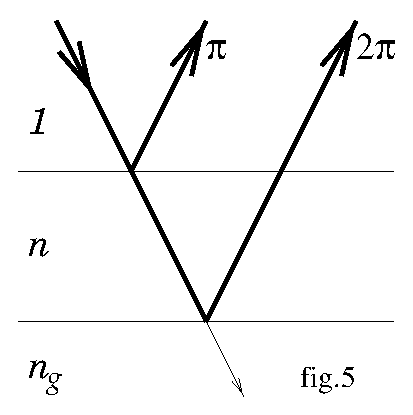
\includegraphics[clip,height=35mm,width=35mm]{1997phy2-5.eps}\hspace{15mm}
\includegraphics[clip,height=35mm,width=35mm]{1997phy2-6.eps}
\end{center}

\parbox[t]{50mm}{\vspace*{-5mm}
\begin{center}
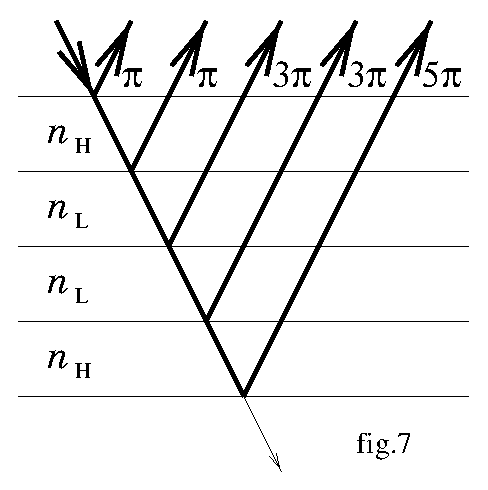
\includegraphics[clip,height=40mm,width=40mm]{1997phy2-7.eps}
\end{center}}\parbox[t]{110mm}{それで、今度は屈折率の大きいもの($n_{\rm{H}}$)を小さいもの($n_{\rm{L}}$)を交互に重ねる(fig.7)。左図のように重ねた多層膜は、反射増加膜として働く。実際、このような高反射率透明多層膜は、膜の数が十分に増えると、広い波長範囲にわたって、ほぼ一様な高反射率を示すようになり、このとき、同時に性能も向上し、反射率99%以上のものを作ることができる。ちなみに、普通の銀膜をつかった鏡の反射率は高々96%である。 

{\bf{[注]}} 波長$1/4$の光学的厚さをもつ薄膜を何層か重ねて、その内部で生じる干渉を利用して、特定の波長領域の光のみを透過、または、反射するフィルターのことを、干渉フィルターと呼ぶ。}



\end{subanswers}
\end{answer}
\end{document}
